% Copyright 2020 by Robert Hildebrand
%This work is licensed under a
%Creative Commons Attribution-ShareAlike 4.0 International License (CC BY-SA 4.0)
%See http://creativecommons.org/licenses/by-sa/4.0/

\documentclass[../open-optimization/open-optimization.tex]{subfiles}

\begin{document}

\chapter{Algorithms to Solve Integer Programs}
\label{sec:IP-algorithms}
\section{LP to solve IP}

Recall that he linear relaxation of an integer program is the linear programming problem after removing the integrality constraints
$$
\begin{array}{rlclr}
\text{ Integer Program:} & & & \text{Linear Relaxation:}\\
\max \ & z_{IP} = c^\top x & \hspace{3cm} & & \max \  z_{LP} = c^\top x \\
& Ax \leq b & & & Ax \leq b\\
& \tred{x \in \Z^n} & & & \tblue{x \in \R^n}
\end{array}
$$

\begin{theorem}[LP Bounds]
It always holds that 
\begin{equation}
z^*_{IP} \leq z^*_{LP}.
\end{equation}
Furthermore, if $x^*_{LP}$ is integral (feasible for the integer program), then 
\begin{equation}
x^*_{LP} = x^*_{IP} \ \ \text{ and } z^*_{LP} = z^*_{IP}.
\end{equation}
\end{theorem}

\begin{example}

%%second column
%\begin{minipage}[t]{0.1\textwidth}
%\includegraphics[scale = 0.3]{LP-equals-IP.png}
%\end{minipage}
%
%Here is some text.\\
% first column
\begin{minipage}[t]{0.5\textwidth}
Consider the problem 
\begin{align*}
\max z = & 3x_1 + 2x_1\\
& 2x_1 + x_2 \leq 6\\
& x_1, x_2 \geq 0; x_1, x_2 \text{ integer}
\end{align*}
\end{minipage}
%
%second column
\begin{minipage}[t]{0.4\textwidth}
%This is the graph
\end{minipage}
\end{example}


%  \includegraphics[width=2cm,height=2cm]{LP-equals-IP.png}\fbox{\LARGE J}
  
  
  \subsection{Rounding LP Solution can be bad!}
  
  Consider the two variable knapsack problem
  \begin{align}
  \max   3x_1 + 100 x_2\\
              x_1  + 10 x_2 \leq 10\\
              x_i \in \{0,1\} \text{ for } i=1,2.
  \end{align}
  
  Then $x^*_{LP} = [1, 0.99]$ and $z^*_{LP} = 1\cdot 3 + 0.99\cdot 100 = 3 + 99 = 102.$
  
  But $x^*_{IP} = [0,1]$ with $z^*_{IP} = 0\cdot 3 + 1 \cdot 100 = 100$.
  
  Suppose that we rounded the LP solution.  
  
  $x^*_{LP-Rounded-Down} = [1,0]$.  Then $z^*_{LP-Rounded-Down} = 1\cdot 3 = 3$.  Which is a terrible solution!
  
  
  How can we avoid this issue?
  
  
  Cool trick!   Using two different strategies gives you at least a 1/2 approximation to the optimal solution.
  
  
  \subsection{Rounding LP solution can be infeasible!}
  Now only could it produce a poor solution, it is not always clear how to round to a feasible solution.  
  
\subsection{Fractional Knapsack}
The fractional knapsack problem has an exact greedy algorithm.

\begin{itemize}
\item \href{https://www.youtube.com/watch?time_continue=424&v=m1p-eWxrt6g}{Youtube!}
\item \href{https://www.geeksforgeeks.org/fractional-knapsack-problem/}{Blog}
\end{itemize}

\section{Branch and Bound}

See \href{http://web.tecnico.ulisboa.pt/mcasquilho/compute/_linpro/TaylorB_module_c.pdf}{Module by Miguel Casquilho} for some nice notes on branch and bound.


\subsection{Algorithm}


\begin{algorithm}[H]
\algorithmicrequire{Integer Linear Problem with max objective}\\
\algorithmicensure{Exact Optimal Solution $x^*$}
\caption{Branch and Bound - Maximization}\label{alg:branch-and-bound-max}
\begin{algorithmic}[1]
	\State Set $LB = - \infty$.
 	\State Solve LP relaxation. 
	\begin{algsubstates}
        		\State If $x^*$ is integer, stop!
        		\State Otherwise, choose fractional entry $x_i^*$ and branch onto subproblems:\ \ \ \hspace{3cm}  (i) $x_i \leq \lfloor x^*_i \rfloor$ and (ii) $x_i \geq \lceil x^*_i \rceil$.        \end{algsubstates}
	\State Solve LP relaxation of any subproblem.
		\begin{algsubstates}
		\State If LP relaxation is infeasible, prune this node as "Infeasible"
        		\State If $z^* < LB$, prune this node as "Suboptimal"
		\State $x^*$ is integer, prune this nodes as "Integer" and update $LB = \max(LB, z^*)$.
		\State Otherwise, choose fractional entry $x_i^*$ and branch onto subproblems:\ \ \ \hspace{3cm}  (i) $x_i \leq \lfloor x^*_i \rfloor$ and (ii) $x_i \geq \lceil x^*_i \rceil$.     Return to step 2 until all subproblems are pruned.
      \end{algsubstates}
      \State Return best integer solution found.
	\end{algorithmic}
\end{algorithm}

%\url{http://www.sce.carleton.ca/faculty/chinneck/po/Chapter12.pdf}
%
%\url{http://www.sce.carleton.ca/faculty/chinneck/po/Chapter13.pdf}
%
%\includegraphics[scale = 0.5]{branch-and-bound-problem}
%
%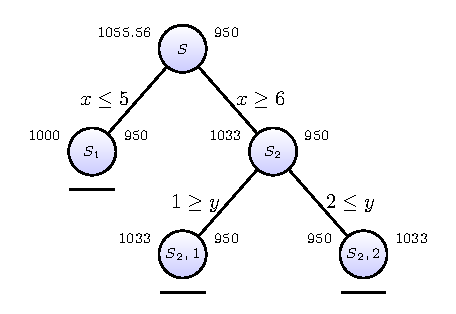
\includegraphics[scale = 0.5]{branch-and-bound}




Here is an example of branching on general integer variables.

\begin{example}{}{}
Consider the two variable example with
 
 \begin{align*}
 \max & -3x_1 + 4x_2\\
 & 2x_1 + 2 x_2 \leq 13\\
 & -8 x_1 + 10x_2 \leq 41\\
 & 9x_1 + 5x_2 \leq 45\\
 & 0 \leq x_1 \leq 10, \text{ integer }\\
 & 0 \leq x_2 \leq 10, \text{ integer }
 \end{align*}
$x =  [1.33, 5.167]  obj =  16.664$\\
\noindent 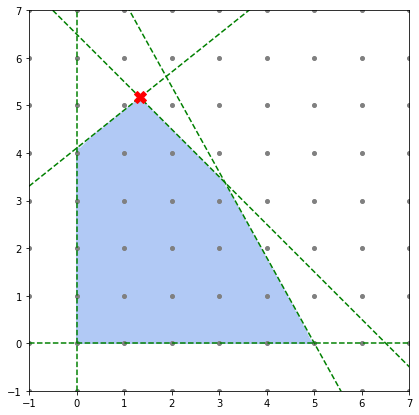
\includegraphics[scale = 0.3]{branch-and-bound1}\\
$x =  [1,  4.9]  obj =  16.5998$\\
$x =  [2,  4.5]  obj =  12.0$\\
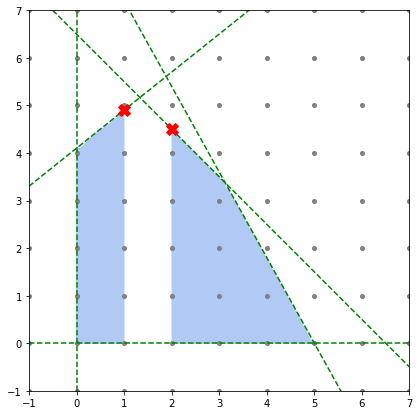
\includegraphics[scale = 0.3]{branch-and-bound2}\\
Infeasible Region\\
$x =  [0. 4.]  obj =  16.0$\\
$x =  [2.  4.5]  obj =  12.0$\\
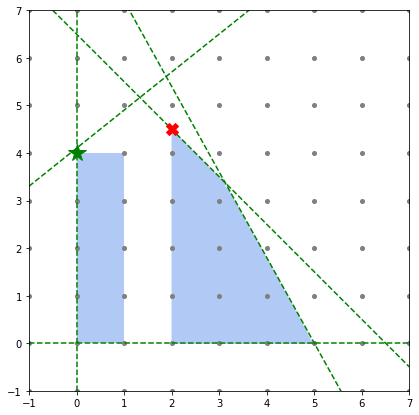
\includegraphics[scale = 0.3]{branch-and-bound3}\\

\end{example}



\subsection{Knapsack Problem  and 0/1 branching}

Consider the problem 

\begin{align*}
\max \quad & 16x_1 + 22x_2 + 12x_3 + 8 x_4\\
\st & 5x_1 + 7x_2 + 4x_3 + 3x_4 \leq 14\\
& 0 \leq x_i \leq 1 \ \ i=1,2,3,4\\
& x_i \in \{0,1\} \ \ i=1,2,3,4
\end{align*}

\textbf{Question: What is the optimal solution if we remove the binary constraints?}




\begin{align*}
\max \quad & c_1 x_1 + c_2 x_2 + c_3 x_3 + c_4 x_4\\
\st & a_1 x_1 + a_2 x_2 + a_3 x_3 + a_4 x_4 \leq b\\
& 0 \leq x_i \leq 1 \ \ i=1,2,3,4\\
\end{align*}

\textbf{Question: How do I find the solution to this problem?}


\begin{align*}
\max \quad & c_1 x_1 + c_2 x_2 + c_3 x_3 + c_4 x_4\\
\st & (a_1 - A)x_1 + (a_2-A) x_2 + (a_3-A) x_3 + (a_4-A) x_4 \leq 0\\
& 0 \leq x_i \leq m_i \ \ i=1,2,3,4\\
\end{align*}

\textbf{Question: How do I find the solution to this problem?}



Consider the problem 

\begin{align*}
\max \quad & 16x_1 + 22x_2 + 12x_3 + 8 x_4\\
\st & 5x_1 + 7x_2 + 4x_3 + 3x_4 \leq 14\\
& 0 \leq x_i \leq 1 \ \ i=1,2,3,4\\
& x_i \in \{0,1\} \ \ i=1,2,3,4
\end{align*}

We can solve this problem with branch and bound.


The optimal solution was found at $t=5$ at subproblem 6 to be $x^* = (0,1,1,1)$, $z^* = 42$.



\textbf{Example: Binary Knapsack}
%\begin{example}{Binary Knapsack Example}{}
Solve the following problem with branch and bound.
\begin{align*}
\max\ \ \   z&=11x_1+15x_2+6x_3+2x_4 + x_5\\
\text{Subject to:} \ \ \ 	 &5x_1+7x_2+4x_3+3x_4 + 15x_5\leq15\\
		&x_i  \text{  binary},i=1,\dots,4
\end{align*}

% Branch and bound tree for maximize knapsack
\tikzset{
  S/.style = {draw, rectangle, rounded corners=0.1cm, minimum size = 8mm,  top color=blue!10, bottom color=blue!10},% top color=white, bottom color=blue!20},
}
     \begin{tikzpicture}[-,thick]
\node[S,sibling distance=5cm, level distance=1.3cm, align=left, label={[blue]left:$t = 1$}, label = {above:\textbf{Root Node}}] 
	{$x^* = (1,1,0.75,0,0) $\\ $z^* = 30.5$\\ $ LB = -\infty$} 
	[sibling distance=7cm, level distance=2.8cm,align=left]
	%
     	child {node[S, label={[blue]left:$t = 2$}, label = {[red]below: \rule{3cm}{0.8pt} \\ \centering Integer}] 
     		{$x^* = (1,1,0,1,0) $\\$z^* = 28$\\$ LB = 28$}
		[sibling distance=2.5cm, level distance=2.8cm,align=left]
   		edge from parent node[left] {$x_3 = 0$}
   }
     child {node[S, label={[blue]right:$t =3$}] 
     		{$x^* = (1,0.857,1,0,0) $\\$z^* = 29.857$\\$ LB = 28$}
		[sibling distance=5cm, level distance=2.8cm,align=left]
		%
     		child {node[S, label={[blue]left:$t = 4$}, label = {[red]below: \rule{3cm}{0.8pt} \\ \centering Suboptimal}] {$x^* = (1,0,1,1,0.2)$\\$z^* = 19.2$\\$ LB = 28$}
     			edge from parent node[left] {$x_2 = 0$}}
     		child {node[S, label={[blue]right:$t =5$}] {$x^* = (0.8,1,1,0,0)$\\$z^* = 29.8$\\$ LB = 28$}[sibling distance=5cm, level distance=2.8cm,align=left]
			child {node[S, label={[blue]left:$t =6$}, , label = {[red]below: \rule{3cm}{0.8pt} \\ \centering Suboptimal}] {$x^* = (0,1,1,1,0.067)$\\$z^* = 23.067$\\$ LB = 28$}[sibling distance=5cm, level distance=2.8cm,align=left]
				edge from parent node[left] {$x_1 = 0$}
				}
			child {node[S, label={[blue]right:$t =7$}, label = {[red]below: \rule{3cm}{0.8pt} \\ \centering Infeasible}] {\\ Infeasible \hspace{3cm} \\ }[sibling distance=5cm, level distance=2.8cm,align=left]
				edge from parent node[right] {$x_1 = 1$}
				}
     			edge from parent node[right] {$x_2 = 1$}
			}
   		edge from parent node[right] {$x_3 = 1$}
   };

     \end{tikzpicture}


%\end{example}

\subsection{Traveling Salesman Problem solution via Branching}


\begin{todo}
Describe solving TSP via a generalized branching method that removes subtours (instead of adding constraints).
\end{todo}




\section{Cutting Planes}
Cutting planes are inequalities $\pi^\top x \leq \pi_0$ that are valid for the feasible integer solutions that the cut off part of the LP relaxation.  Cutting planes can create a tighter description of the feasible region that allows for the optimal solution to be obtained by simply solving a strengthened linear relaxation. 

The cutting plane procedure, as demonstrated in Figure~\ref{fig:cutting-plane-procudure}.  The procedure is as follows:
\begin{enumerate}
\item Solve the current LP relaxation.
\item If solution is integral, then return that solution.  STOP
\item Add a cutting plane (or many cutting planes) that cut off the LP-optimal solution.
\item Return to Step 1.
\end{enumerate}

\begin{figure}[H]
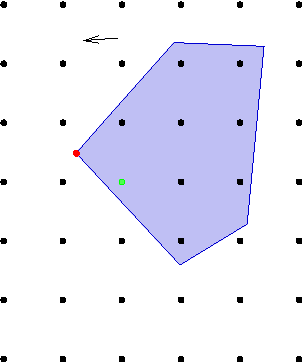
\includegraphics[scale = 0.4]{figureCutttingPlane1}
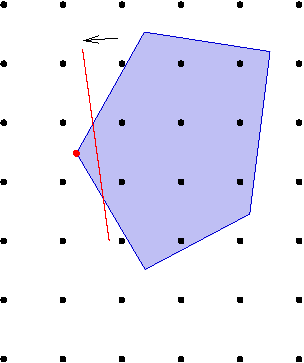
\includegraphics[scale = 0.4]{figureCutttingPlane2}
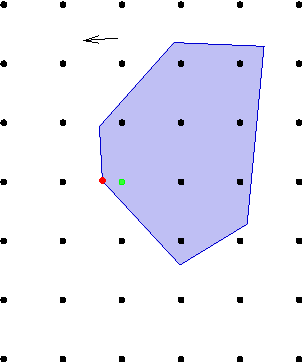
\includegraphics[scale = 0.4]{figureCutttingPlane3}
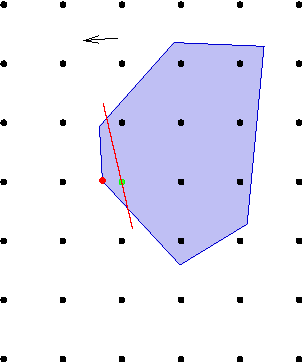
\includegraphics[scale = 0.4]{figureCutttingPlane4}
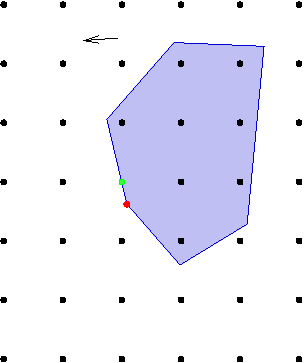
\includegraphics[scale = 0.4]{figureCutttingPlane5}
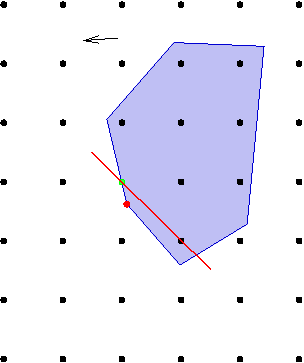
\includegraphics[scale = 0.4]{figureCutttingPlane6}
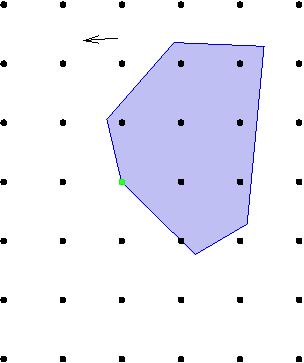
\includegraphics[scale = 0.4]{figureCutttingPlane7}
\caption{The cutting plane procedure.}
\label{fig:cutting-plane-procudure}
\end{figure}

In practice, this procedure is integrated in some with with branch and bound and also other primal heuristics.

%\begin{table}
%\centering\begin{tabular}{|>{\centering\arraybackslash}m{3cm}|>{\centering\arraybackslash}m{5cm}|} \hline\textbf{Topic} & \textbf{Paragraph} \\\hline \hlineTopic 1 & This is a paragraph. This is a paragraph. This is a paragraph.\\\hline\end{tabular}
%\end{table}

\begin{table}[h]
\centering\begin{tabular}{>{\centering\arraybackslash}m{5cm}>{\centering\arraybackslash}m{10cm}}
 \hline
\textbf{Model} & \textbf{LP Solution} \\\hline \hline

$$
\begin{array}{lrl}
\max \ & x_1 + x_2\\
\text{subject to  } &  -2x_1 + x_2 &\leq 0.5\\
& x_1 + 2x_2 &\leq 10.5\\
& x_1 - x_2 &\leq 0.5\\
& - 2x_1 - x_2 &\leq -2
\end{array} 
$$
&
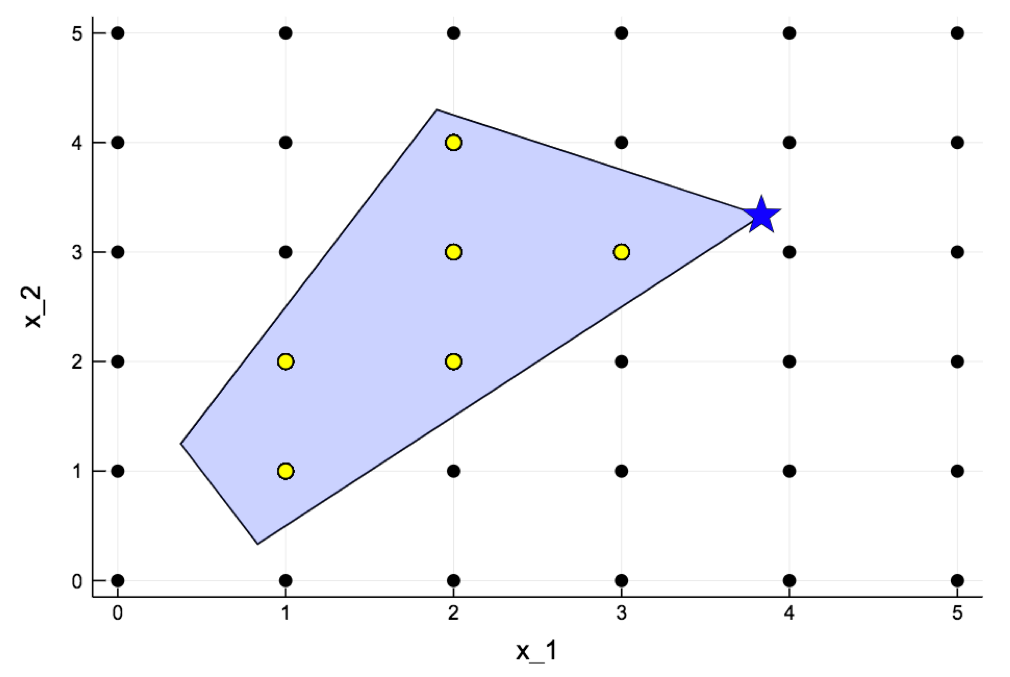
\includegraphics[scale = 0.5]{cutting-plane-1-picture}\\
$$
\begin{array}{lrl}
\max \ & x_1 + x_2\\
\text{subject to  } &  -2x_1 + x_2 &\leq 0.5\\
& x_1 + 2x_2 &\leq 10.5\\
& x_1 - x_2 &\leq 0.5\\
& - 2x_1 - x_2 &\leq -2\\
& \tred{x_1} &\tred{\leq 3}
\end{array} 
$$
&
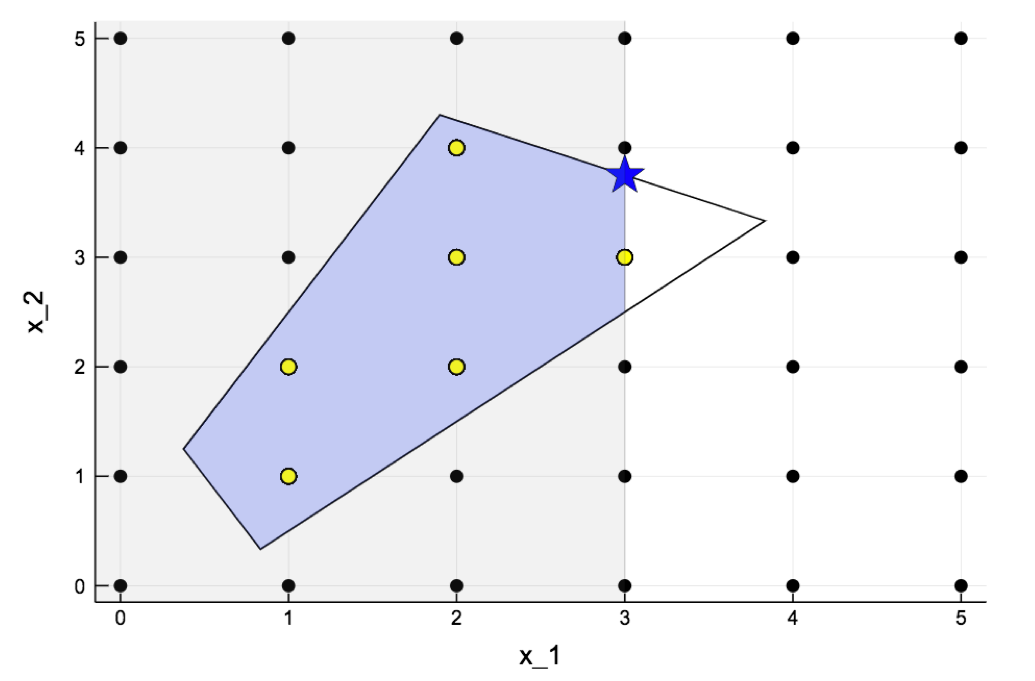
\includegraphics[scale = 0.5]{cutting-plane-2-picture}\\
$$
\begin{array}{lrl}
\max \ & x_1 + x_2\\
\text{subject to  } &  -2x_1 + x_2 &\leq 0.5\\
& x_1 + 2x_2 &\leq 10.5\\
& x_1 - x_2 &\leq 0.5\\
& - 2x_1 - x_2 &\leq -2\\
& \tred{x_1} & \tred{\leq 3}\\
& \tred{x_1 + x_2} & \tred{\leq 6}
\end{array} 
$$
&
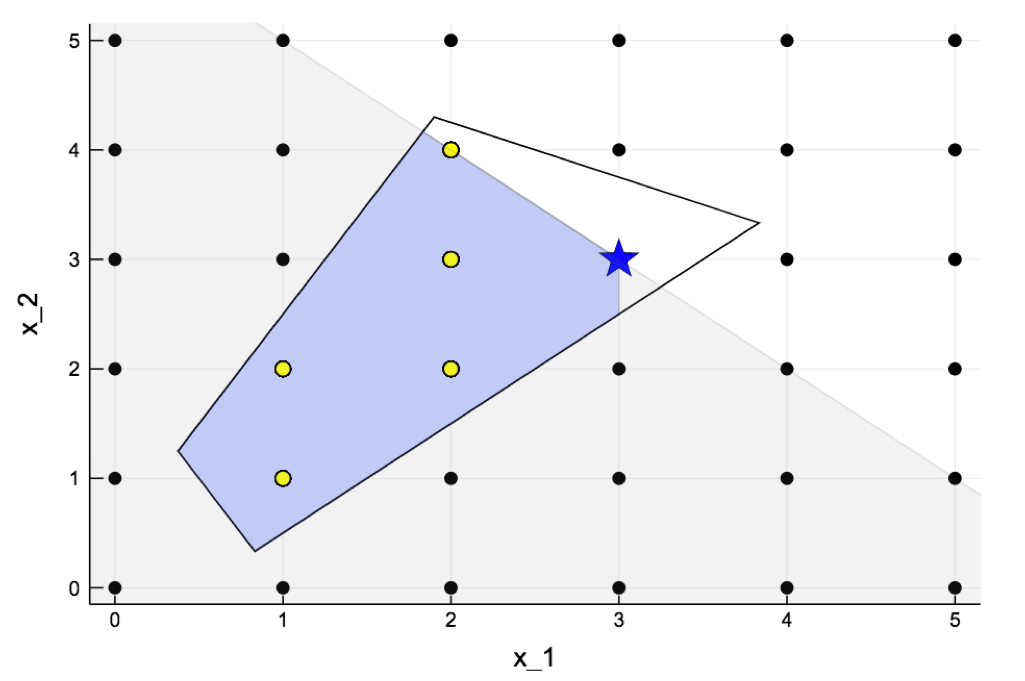
\includegraphics[scale = 0.5]{cutting-plane-3-picture}\\
\hline
 \end{tabular}
\end{table}


\subsection{Chv\'atal Cuts}


Chv\'atal Cuts are a general technique to produce new inequalities that are valid for feasible integer points.  


\begin{general}{Chv\'atal Cuts}{}
Suppose 
\begin{equation}
a_1 x_1 + \dots + a_n x_n \leq d
\end{equation}
is a valid inequality for the polyhedron $P = \{ x \in \R^n : Ax \leq b, x \geq 0\}$, then 
\begin{equation}
\label{eq:chvatal}
\lfloor a_1\rfloor x_1 + \dots + \lfloor a_n\rfloor  x_n \leq \lfloor d\rfloor
\end{equation}
is valid for the integer points in $P$, that is, it is valid for the set $P \cap \Z^n$.  Equation~\eqref{eq:chvatal} is called a Chv\'atal Cut.
\end{general}


We will illustrate this idea with an example.


\begin{example}{}{}
Recall example~\ref{ex:min-coins}.  The model was\\
\textbf{Model}
\begin{align*}
\min \quad & p + n + d + q & \text{ total number of coins used}\\
\text{ s.t. } \quad & p + 5n + 10d + 25 q = 83 & \text{sums to } 83 \cent\\
& p,d,n,q \in \Z_+ & \text{each is a non-negative integer}
\end{align*}

From the equality constraint we can derive several inequalities.
\begin{enumerate}
\item Divide by 25 and round down both sides:
\[
\frac{p + 5n + 10d + 25 q}{25} = 83/25 \quad \Rightarrow \quad q \leq 3 
\]
\item Divide by 10 and round down both sides:
\[
\frac{p + 5n + 10d + 25 q}{10} = 83/10 \quad \Rightarrow \quad d + 2q \leq 8 
\]
\item Divide by 5 and round down both sides:
\[
\frac{p + 5n + 10d + 25 q}{10} = 83/5 \quad \Rightarrow \quad n + 2d  + 5q \leq 16
\]
\item Multiply by 0.12 and round down both sides:
\[
0.12(p + 5n + 10d + 25 q = 0.12 (83) \quad \Rightarrow \quad d  + 3q \leq 9
\]
\end{enumerate}
These new inequalities are all valid for the integer solutions.  Consider the new model:\\

\textbf{New Model}
\begin{align*}
\min \quad & p + n + d + q & \text{ total number of coins used}\\
\text{ s.t. } \quad & p + 5n + 10d + 25 q = 83 & \text{sums to } 83 \cent\\
& q \leq 3\\
& d + 2q \leq 8 \\
& n + 2d  + 5q \leq 16\\
& d  + 3q \leq 9\\
& p,d,n,q \in \Z_+ & \text{each is a non-negative integer}
\end{align*}

The solution to the LP relaxation is exactly $q = 3, d = 0, n = 1, p = 3$, which is an integral feasible solution, and hence it is an optimal solution.
\end{example}


\subsection{Gomory Cuts}
Gomory cuts are a type of Chv\'atal cut that is derived from the simplex tableau.  Specifically, suppose that 
\begin{equation}
\label{eq:tableau-row}
 x_i + \sum_{i\in N} \tilde a_i x_i = \tilde b_i
\end{equation}
is an equation in the optimal simplex tableau. 

\begin{general}{Gomory Cut}{}
The Gomory cut corresponding to the tableau row ~\eqref{eq:tableau-row} is

\begin{equation}
\label{eq:gomory-cut}
\sum_{i\in N} (\tilde a_i - \lfloor \tilde a_i \rfloor) x_i \geq \tilde b_i - \lfloor \tilde b_i\rfloor
\end{equation}


\end{general}


We will solve the following problem using only Gomory Cuts.
\begin{equation*}
\begin{array}{lrcl}
\min & x_1 - 2x_2\\
\st & -4x_1 + 6x_2  & \leq & 9\\
& x_1 + x_2   & \leq & 4\\
& x \geq 0 & , & x_1,x_2 \in \Z
\end{array}
\end{equation*}

\textbf{Step 1:} The first thing to do is to put this into standard from by appending slack variables.
\begin{equation}
\label{eq:gomory-standard-form}
\begin{array}{lrcl}
\min & x_1 - 2x_2\\
\st & -4x_1 + 6x_2 + s_1 & = & 9\\
& x_1 + x_2 + s_2  & = & 4\\
& x \geq 0 & , & x_1,x_2 \in \Z
\end{array}
\end{equation}

We can apply the simplex method to solve the LP relaxation.\\
\begin{tabular}{cc}
Initial Basis & 
%\begin{center}
\begin{tabular}{|lr|rrrr|}
\hline
 Basis & RHS & $x_1$ & $x_2$ & $s_1$ & $s_2$ \\
 \hline
 $z$     & 0.0 & 1.0   & -2.0  & 0.0   & 0.0   \\
 \hline
 $s_1$ & 9.0 & -4.0  & 6.0   & 1.0   & 0.0   \\
 $s_2$ & 4.0 & 1.0   & 1.0   & 0.0   & 1.0   \\
\hline
\end{tabular}\\
%\end{center}\\
\vdots & \vdots  \\
Optimal Basis & 
%Pivoting to the optimal basis, we have
%\begin{center}
\begin{tabular}{|lr|rrrr|}
\hline
 Basis & RHS  & $x_1$ & $x_2$ & $s_1$ & $s_2$ \\
 \hline
 $z$     & -3.5 & 0.0   & 0.0   & 0.3   & 0.2   \\
 \hline
 $x_1$ & 1.5  & 1.0   & 0.0   & -0.1  & 0.6   \\
 $x_2$ & 2.5  & 0.0   & 1.0   & 0.1   & 0.4   \\
\hline
\end{tabular}
%\end{center}
\end{tabular}

This LP relaxation produces the fractional basic solution $x_{LP} = (1.5, 2.5)$.


\begin{example}\textbf{(Gomory cut  removes LP solution)}{}\\
 We now identify an integer variable $x_i$ that has a fractional basic solution.  Since both variables have fractional values, we can choose either row to make a cut.  Let's focus on the row corresponding to $x_1$.

The row from the tableau expresses the equation 
\begin{equation}
x_1 - 0.1 s_1 + -0.6 s_2 = 1.5.
\end{equation}

Applying the Gomory Cut~\eqref{eq:gomory-cut}, we have the inequality 
\begin{equation}
\label{eq:gomory-cut-ex1}
0.9 s_1 + 0.4 s_2 \geq 0.5.
\end{equation}

The current LP solution is $(x_{LP}, s_{LP}) = (1.5, 2.5,0,0)$.  Trivially, since $s_1, s_2 = 0$, the inequality is violated.
\end{example}

\begin{example}\textbf{(Gomory Cut in Original Space)}\\

The Gomory Cut~\eqref{eq:gomory-cut-ex1} can be rewritten in the original variables using the equations from~\eqref{eq:gomory-standard-form}.  That is, we can use the equations
\begin{equation}
\label{eq:gomory-standard-form-equations}
\begin{array}{lrcl}
 & s_1 & = & 9 + 4x_1 - 6x_2\\
&s_2  & = & 4 - x_1 - x_2,
\end{array}
\end{equation}
which transforms the Gomory cut into the original variables to create the inequality
\begin{equation*}
\label{eq:gomory-cut-ex1-original}
0.9 (9 + 4x_1 - 6x_2) + 0.4(4 - x_1 - x_2) \geq 0.5.
\end{equation*}
or equivalently
\begin{equation}
\label{eq:gomory-cut-ex1-original}
- 3.2 x_1 + 5.8 x_2 \leq 9.2.
\end{equation}
%\textbf{Check!} We can now check if this inequality cuts off the current LP optimal solution.
%To see this, let's plug in $(x_{LP}, s_{LP}) = (1.5, 2.5,0,0)$.
%
%\begin{equation}
%\label{eq:gomory-cut-ex1-original}
%- 3.2 x_1 + 5.8 x_2 = - 3.2 (1.5) + 5.8 (2.5) = 9.7 > 9.2
%\end{equation}
%Thus, this LP solution is violated by the new Gomory Cut.

As you can see, this inequality does cut off the current LP relaxation.
%\includegraphics[scale = 0.5]{this-graphic.}

\end{example}


\begin{example}{\textbf{(Gomory  cuts plus new tableau)}}{}
Now we add the slack variable $s_3 \geq 0$ to make the equation
\begin{equation}
0.9 s_1 + 0.4 s_2 - s_3 = 0.5.
\end{equation}


\end{example}


Next, we need to solve the linear programming relaxation (where we assume the variables are continuous).




\section{Branching Rules}
There is a few clever ideas out there on how to choose which variables to branch on.  We will not go into this here.  But for the interested reader, look into 
\begin{itemize}
\item Strong Branching
\item Pseudo-cost Branching
\end{itemize}

\section{Lagrangian Relaxation for Branch and Bound}

At each note in the branch and bound tree, we want to bound the objective value.  One way to get a a good bound can be using the Lagrangian. 

See~\cite{Fisher2004}  \href{https://my.eng.utah.edu/~kalla/phy_des/lagrange-relax-tutorial-fisher.pdf}{(link)} for a description of this.



\section{Benders Decomposition}
\href{https://www.juliaopt.org/notebooks/Shuvomoy%20-%20Benders%20decomposition.html}{Benders Decomposition - Julia Opt}

\section{Literature}

\end{document}
